%%%%%%%%%%%%%%%%%%%%%%%%%%%%%%%%%%%%%%%%%%%%%%%%%%%%%%%%%%%%%%%%%
% Dissertacao de Mestrado / Dept Fisica, CFM, UFSC              %
% Lacerda@UFSC - 2013                                           %
%%%%%%%%%%%%%%%%%%%%%%%%%%%%%%%%%%%%%%%%%%%%%%%%%%%%%%%%%%%%%%%%%

%:::::::::::::::::::::::::::::::::::::::::::::::::::::::::::::::%
%                                                               %
%                          Capítulo 3                           %
%                                                               %
%:::::::::::::::::::::::::::::::::::::::::::::::::::::::::::::::%

%***************************************************************%
%                                                               %
%                      PCA e Tomografia PCA                     %
%                                                               %
%***************************************************************%

\chapter{PCA e Tomografia PCA}
\label{sec:PCAeTomoPCA}

De medidas fisiológicas, como pulsação e respiração, até reconhecimento de padrões em sistemas complexos como
reconhecimento facial e criptografia, passando por compactação de imagem, neurosciência e redução de ruídos em dados,
podemos ver atuação de técnicas de PCA. Neste capítulo revisamos os fundamentos matemáticos do PCA e de sua versao para
cubos de dados (Tomografia PCA).

%***************************************************************% 
%                                                               %
%                              PCA                              %
%                                                               % 
%***************************************************************%

\section{Principal Component Analisys}
\label{sec:PCAeTomoPCA:PCA}

Baseada em encontrar os eixos com maiores variâncias em um conjunto de variáveis (no nosso caso, fluxos por lambda e por
zona espacial), a técnica de PCA vem sendo de grande utilidade quando o assunto é estatística com muitas variáveis.
Através de operações relativamente simples usando álgebra linear, é feita uma rotação na base de dados original, gerando
uma nova base ortonormal não correlacionada através de um conjunto de autovalores e autovetores.

Existem diversas formas de se calcular essa base final. A prova matemática que você pode obter essa base é feita através
de multiplicadores de Lagrange, calculando os autovetores ($\mathbf{e}{}_k$) e autovalores ($\Lambda_k$) que maximizam o
valor de $\mathbf{e}{}_k^T \cdot \mathbf{C}{}_{cov} \cdot \mathbf{e}{}_k$ (ver Eq. \ref{eq:PCA:covMatrix}) sujeito à
restrição de que um autovetor deve ser ortogonal a qualquer outro da base ($\mathbf{e}{}_i^T \mathbf{e}{}_j = 0$) e que
todos devem ser normalizados ($\mathbf{e}{}_i{}^T \mathbf{e}{}_i = 1$) \citep[][p. 5-6]{JolliffePCA1986}. No caso caso
de PCA com espectros, cada um pode ser represtado como um ponto num espaço com dimensão $N_\lambda$. Vários espectros
formam uma núvem de pontos nesse espaço. Assim, encontramos quais são os eixos mais significativos desse espaço em
relação à variância, sujeitos às restrições acima. Fazemos esse cálculo encontrando os autovetores e autovalores da
matriz de covariância desse espaço (a matriz tem dimensão $N_\lambda \times N_\lambda$) usando a biblioteca científica
\texttt{SciPy}\footnote{\url{http://scipy.org/}} (\ref{fig:PCA:covMatrix}), que encontra os autovetores e autovalores
dessa matriz.

\subsection{PCA das galáxias do CALIFA}

Conforme a Seção \ref{sec:CALePyC:pipelines} vimos que o cubo de espectros das galáxias do CALIFA estão acessíveis no
PyCASSO separados por zonas, muitas correspondendo a píxeis individuiais e outras a conjuntos de pixeis (zonas de
Voronoi). Os espectros observados estão armazenados em forma de uma matriz ($N_\lambda \times N_z$) com $N_\lambda$
comprimentos de onda e $N_z$ zonas e (\texttt{f\_obs} no PyCASSO). Em nosso trabalho vamos usar a forma transposta dessa
matriz, portanto nossa matriz de espectros está na forma $N_z \times N_\lambda$, como demonstrado na equação abaixo.

\begin{equation}
    \label{eq:PCA:fluxMatrix}
    \textbf{F}{}_{z \lambda} = \left[
    \begin{array}{ccccc}
        F_{z_0 \lambda_0} & F_{z_0 \lambda_1} & F_{z_0 \lambda_2} & ... & F_{z_0 \lambda_{(N_\lambda - 1})} \\
        F_{z_1 \lambda_0} & F_{z_1 \lambda_1} & F_{z_1 \lambda_2} & ... & F_{z_1 \lambda_{(N_\lambda - 1})} \\
        F_{z_2 \lambda_0} & F_{z_2 \lambda_1} & F_{z_2 \lambda_2} & ... & F_{z_2 \lambda_{(N_\lambda - 1})} \\
        ...               & ...               & ...               & ... & ...               \\
        F_{z_{(N_z - 1)} \lambda_0} & F_{z_{(N_z - 1)} \lambda_1} & F_{z_{(N_z - 1)} \lambda_2} & ... & F_{z_{(N_z - 1)}
        \lambda_{(N_\lambda - 1)}}
    \end{array} 
    \right]
\end{equation}

Calculamos então o espectro médio de uma galáxia
\begin{equation}
\langle \textbf{F}{}_\lambda \rangle = \frac{1}{N_z} \sum_{i=0}^{(N_z - 1)} F_{z_i}{}_{\lambda}
\end{equation}
\noindent e então subtraímos a média de todos os espectros
\begin{equation}
\textbf{I}{}_{z \lambda} = \textbf{F}{}_{z \lambda} - \langle \textbf{F}{}_\lambda \rangle
\end{equation}
\noindent para o cálculo da matriz de covariâncias usando um conjunto de dados com média zero:
\begin{equation}
	\label{eq:PCA:covMatrix}
	\mathbf{C}{}_{cov} = \frac{[\mathbf{I}{}_{z \lambda}]^T \cdot \mathbf{I}{}_{z \lambda}}{n - 1}
\end{equation}
\noindent Vemos que a matriz de covariância possui dimensão $N_\lambda \times N_\lambda$.

Agora calculamos os autovalores e autovetores da matriz de covariância. Neste trabalho usamos o nome autoespectro para
designar esses autovetores pois são de uma matriz de covariâncias entre espectros de cada zona. Então ordenamos-os
decrescentemente pelo valor de seus autovalores. Os autoespectros são as componentes principais (PCs) e os autovalores
as respectivas variâncias. Isso feito, temos então o que necessitamos para iniciar o cálculo do Tomograma PCA. Um
exemplo de programa para calcular a matriz de covariâncias e seus autovetores e autovalores usando o \texttt{SciPy} pode
ser visto na Figura \ref{fig:programaCovMatrix}.

\begin{figure}
\begin{python}
# Carregar arquivo FITS com os dados.
from pycasso import fitsQ3DataCube
K = fitsQ3DataCube('K0277_synthesis_suffix.fits')

# Calcular o espectro medio de uma galaxia. 
# K.f_obs tem dimensao (lambda, zona), portanto, 
# fazemos o espectro medio de todas as zonas.
f_obs_mean__l = K.f_obs.mean(axis = 1)

# Subtraimos a media
I_obs__zl = K.f_obs.transpose() - f_obs_mean__l

# Calcular a matrix de convariancia
import scipy as sp
n = K.N_zone
dot_product = sp.dot(I_obs__zl.transpose(), I_obs__zl)
covMat__ll = dot_product / (n - 1.0)   

# Calcular os autovalores e autovetores
w, e = linalg.eigh(covMat__ll)

# Ordenar os autovetores decrescentemente pelo seu autovalor
S = sp.argsort(w)[::-1]
eigval = W[S]
eigvect = e[:, S]
 
\end{python}
	\caption[Exemplo de cálculo de PCA usando o PyCASSO e SciPy.] 
	{Cálculo do procedimento completo de PCA para os espectros observados de uma galáxia do CALIFA usando o PyCASSO e a
	biblioteca científica de Python chamada \texttt{SciPy}. No final do código temos armazenado nos vetores \texttt{eigval}
	e \texttt{eigvect} os autovalores e autovetores da matriz de covariância (\texttt{covMat\_\_ll}) ordenados
	decrescentemente.}
	\label{fig:programaCovMatrix}
\end{figure}

Muitas figuras de PCs e suas utilizações e diferenças nos pré-processamentos serão mostradas nos Capítulos
\ref{sec:PCAaplic} e \ref{sec:result}, juntamente com a Tomografia PCA e as comparações com os parâmetros físicos da
sintese de populações estelares com o \starlight.

%***************************************************************%
%                                                               %
%                        Tomografia PCA                         %
%                                                               %
%***************************************************************%

\section{Tomografia PCA}
\label{sec:PCAeTomoPCA:TomoPCA}

Os autoespectros ($e_k$) da matriz de covariância (PCs) ordenados pela sua variância ($\Lambda_k$) formam uma matriz
($\mathbf{E}{}_{\lambda k}$, de dimensão $N_\lambda \times N_k$, onde $N_k$ é o número de PCs) que serve como base onde
projetamos nossa matriz de observáveis com a média subtraida ($\mathbf{I}{}_{z \lambda}$) através da transformação:

\begin{equation}
	\label{eq:TomoPCA:tomogram2D}
	\mathbf{T}{}_{z k} = \mathbf{I}{}_{z \lambda} \cdot \mathbf{E}{}_{\lambda k}
\end{equation}

Na posse dessa nova matriz transformada e de um mapa que faça a transformação de zona para uma par de coordenada ($z \to
(x, y)$), podemos montar assim uma imagem. Cada imagem funciona como uma ``fatia'' de um cubo de dados expandido na nova
base, assim formando a Tomografia PCA\footnote{\url{http://www.astro.iag.usp.br/~pcatomography/}}, criada e assim
batizada por Steiner em S09, que em seu artigo faz um paralelo com fatias de um espaço tridimensional (tomograma do
corpo humano, por exemplo) ou no espaço de velocidades (Tomografia Doppler). Cada ``fatia'' possui um autoespectro (PC)
relacionado que, em conjunto, trazem novas perspectivas e ideias para a interpretação de ambos.

\section{Exemplos de resultado da Tomagrafia PCA}

Para ilustrar o potencial da tecnica de Tomografia PCA, ilustramos os resultados obtidos em 2 artigos.

\subsection{Descoberta de linhas largas em um LINER}

No artigo citado anteriormente, através do estudo dos autoespectros e suas respectivas imagens do núcleo da galáxia
LINER ({\em Low Ionizations Nuclear Emission-line Region}) NGC 4736, foram encontradas evidências de linhas largas.
Quando temos uma fonte que é capaz de produzir linhas largas no espectro é sinal da existência de um SMBH ({\em Super
Massive Black Hole}). \citet{CidFernandes2004} mostram que, pelo menos em alguns casos, a subtração detalhada das
populações estelares nos espectros ajuda a encontrar linhas largas mais fracas em Seyferts 2, que são aquelas que (por
definição) possuem apenas linhas estreitas, ajudando assim na classificação desses objetos como tipo 1 ou 2. A PCA,
juntamente com a Tomografia PCA, fazem esse papel da subtração das populações estelares sem haver nenhuma
parametrização.

Em S09 estudaram os 8 primeiros autoespectros, escolhidos através de um {\em scree test} (\ref{fig:TomoPCA:scree}), no
qual se verifica a variância de cada PC e toma-se as mais relevantes. O autoespectro com mais variância (no artigo
tratado com E1) possui $99.74\%$ da variância e reproduz comportamento do gás e da população estelar somados (Figura
\ref{fig:TomoPCA:eigspec1}). O segundo contribui com $0.088\%$ para a variância e tem um claro padrão de rotação, tanto
nas linhas do autoespectro quanto na imagem da tomografia (Figura \ref{fig:TomoPCA:eigspec2}). É no terceiro ($0.032\%$
da variância) que mostra evidência clara de uma emissão larga de \Halpha (Figura \ref{fig:TomoPCA:eigspec3}). Essa
assinatura é uma evidência tipica de AGNs de tipo 1.

\begin{figure}
    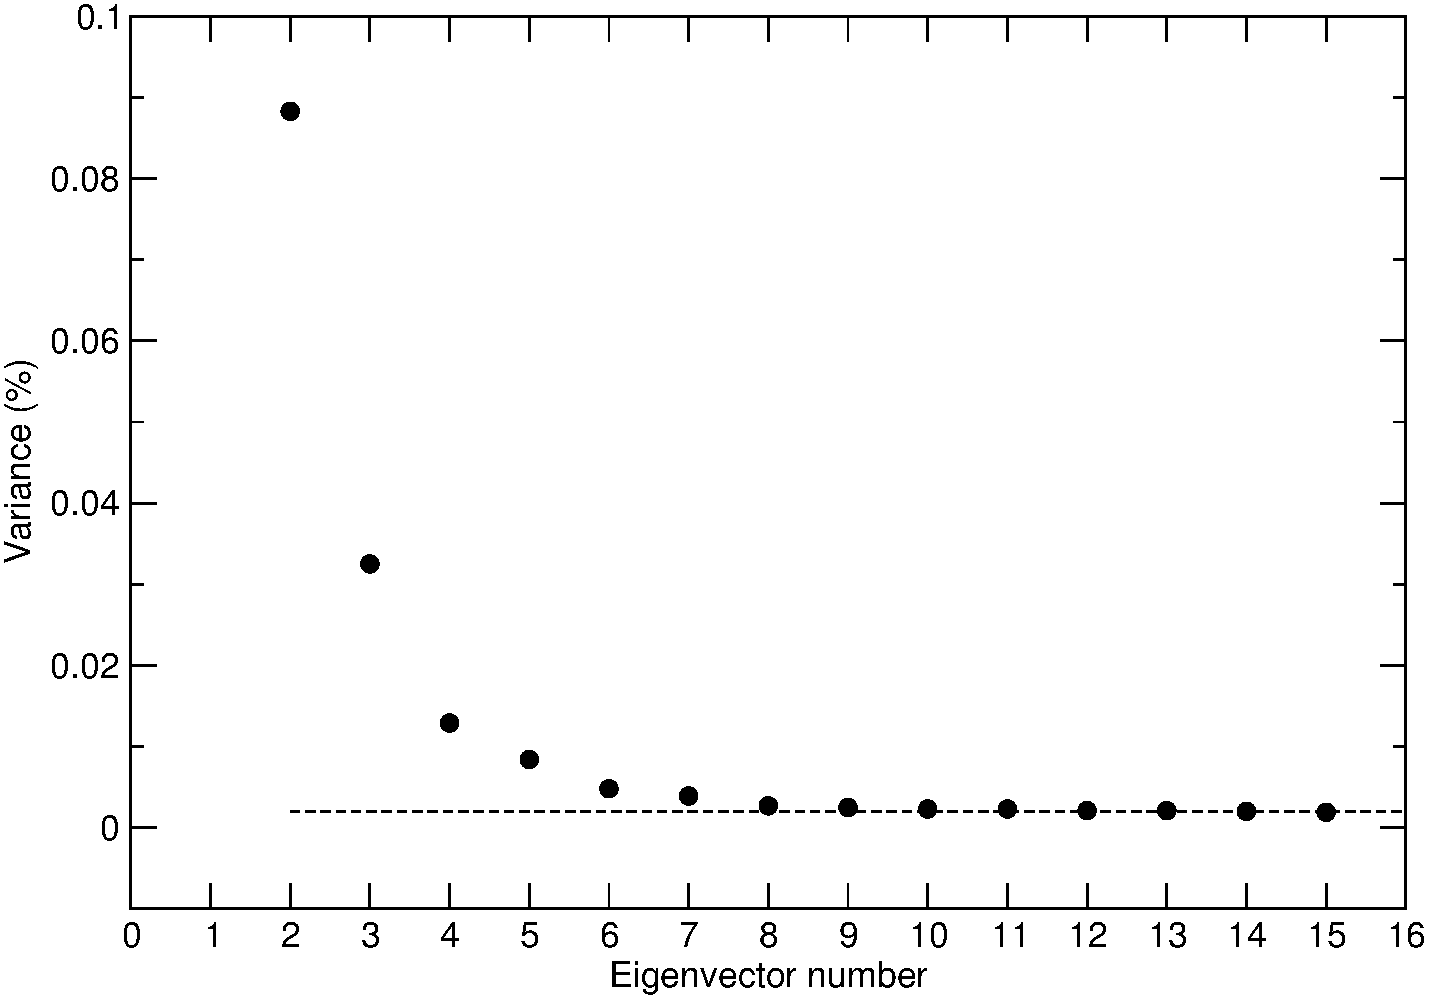
\includegraphics[width=0.7\textwidth]{figuras/figSteiner2009fig1.pdf}
    \caption[{\em Scree test} na galáxia NGC 4736.]
    {Scree test das primeiras 16 PCs do cubo de espectros da região
    central da galáxia NGC 4736. 
    Retirado de \citet[][fig. 1]{Steiner2009}.}
    \label{fig:TomoPCA:scree}
\end{figure}

\begin{figure}
    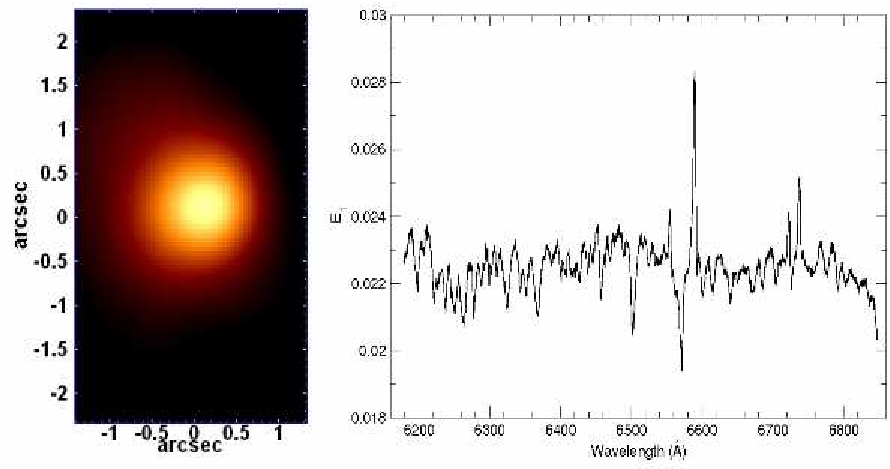
\includegraphics[width=0.9\textwidth]{figuras/figSteiner2009figA1.pdf}
    \caption[Tomograma e autoespectro 1 da galáxia NGC 4736.]
    {Autoespectro 1 e seu respectivo tomograma. Retirado de \citet[][fig.
    A1]{Steiner2009}.}
    \label{fig:TomoPCA:eigspec1}
\end{figure}

\begin{figure}
    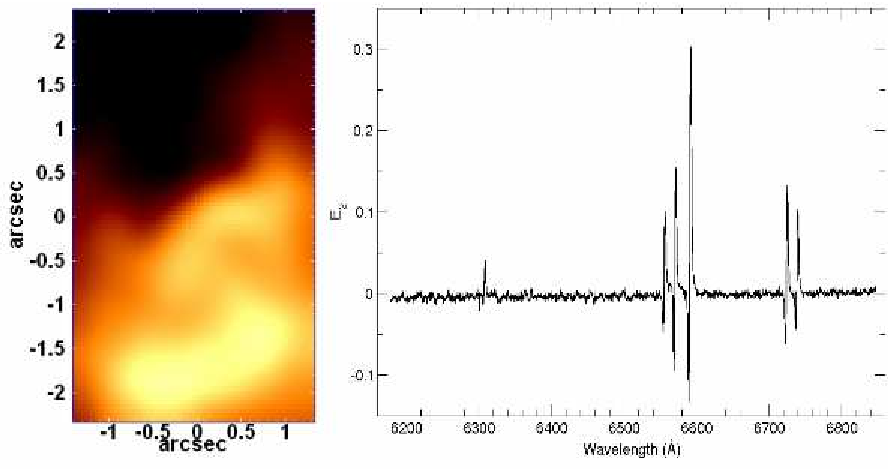
\includegraphics[width=0.9\textwidth]{figuras/figSteiner2009figA2.pdf}
    \caption[Tomograma e autoespectro 2 da galáxia NGC 4736.]
    {Autoespectro 2 e seu respectivo tomograma. Retirado de \citet[][fig.
    A2]{Steiner2009}.}
    \label{fig:TomoPCA:eigspec2}
\end{figure}

\begin{figure}
    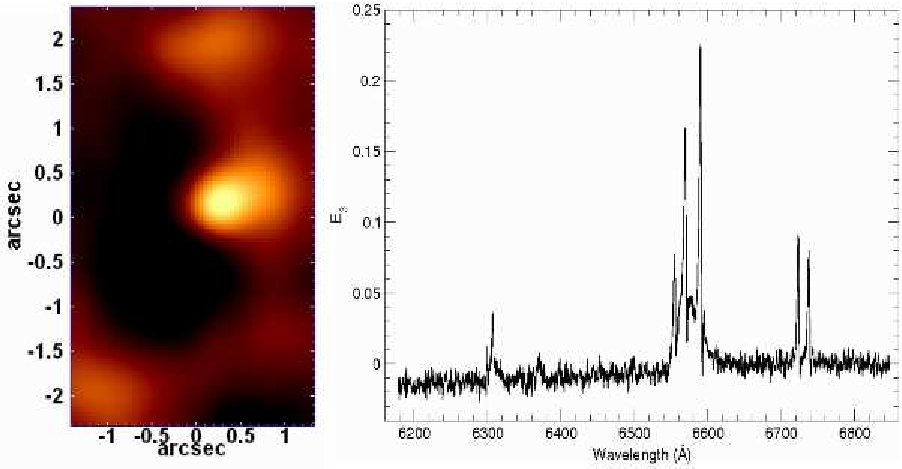
\includegraphics[width=0.9\textwidth]{figuras/figSteiner2009figA3.pdf}
    \caption[Tomograma e autoespectro 3 da galáxia NGC 4736.]
    {Autoespectro 2 e seu respectivo tomograma. Retirado de \citet[][fig.
    A3]{Steiner2009}.}
    \label{fig:TomoPCA:eigspec3}
\end{figure}

\subsection{Reflexao da luz de um AGN escondido em NGC 7097}

{\bf\ojo A FAZER!! \ojo Ricci et al 2011. Figs 3 e 5. vais precisar da minha ajuda para entender esse assunto de reflexao ... le o paper e depois falamos}

\section{Tomografia PCA para dados CALIFA: diferen\c{c}as com respeito a trabalhos anteriores}

Os exemplos acima nos motivam a aplicar esta mesma técnica aos cubos de dados do CALIFA, e o resto desta dissertação
apresenta nossos experimentos nesse sentido. Cumpre ressaltar, contudo, que o tipo de dados que analisaremos difere
bastante dos dados analisados até agora com essa nova ferramenta.

Essas diferenças são tanto de caráter observacional, como metodologico e físico. Para começo de conversa, S09 trabalham
com dados do Gemini (8m) com $3 \times 20$ min de integração, enquanto nossos dados vêm de integrações de tipicamente
?? min no telescópio de 3.5m do observatório de Calar Alto.

Além disso, eles aplicam técnicas de deconvolução das imagens com o algorítmo de Richardson-Lucy. Dado o pequeno {\em
FoV} do IFU do Gemini, o ganho com tais técnicas é perceptível. Não aplicaremos isso no nosso caso porque nosso {\em
FoV} é muito maior, e não esperamos grandes ganhos em resolução espacial com a aplicação de tais técnicas de
deconvolução espacial.

Como dito na Seção \ref{sec:CALePyC:Apresent} a escala e resolução espacial de nossos dados difere brutalmente daquelas
nos trabalhos acima resumidos: $3^{\prime\prime} \times 5^{\prime\prime}$ e resolução de $0.47^{\prime\prime}$ no Gemini
contra $74^{\prime\prime} x 64^{\prime\prime}$ e resolução de $\sim3.7^{\prime\prime}$ no CALIFA. Portanto, o {\em FoV}
estudado por Steiner e colaboradores equivalem a aproximadamente $\sim2$ elementos de resolução do CALIFA! Isto de cara
mostra que a ciência que podemos obter com Tomografia PCA aplicada aos dados do CALIFA não será a mesma que aquela
estudade por S09.

Em resumo, apesar de inspirado diretamente pelos resultados de S09l, este estudo difere muito dos trabalhos deles. Estas
diferenças ficarão evidentes já a partir do próximo capítulo, onde apresentamos nossos primeiros resultados e discutimos
algumas variações com respeito ao processamento de S09, que decidimos fazer para melhor se adequar ao contexto de dados
do CALIFA.

%% End of this chapter